\documentclass{standalone}
\usepackage{tikz}
\usetikzlibrary{patterns}
\usetikzlibrary{positioning}
\usetikzlibrary{patterns, positioning}
\usetikzlibrary{shapes.misc}
\usepackage[outline]{contour}
\contourlength{1.5pt} 
\usepackage[sfdefault]{ClearSans}

\begin{document}
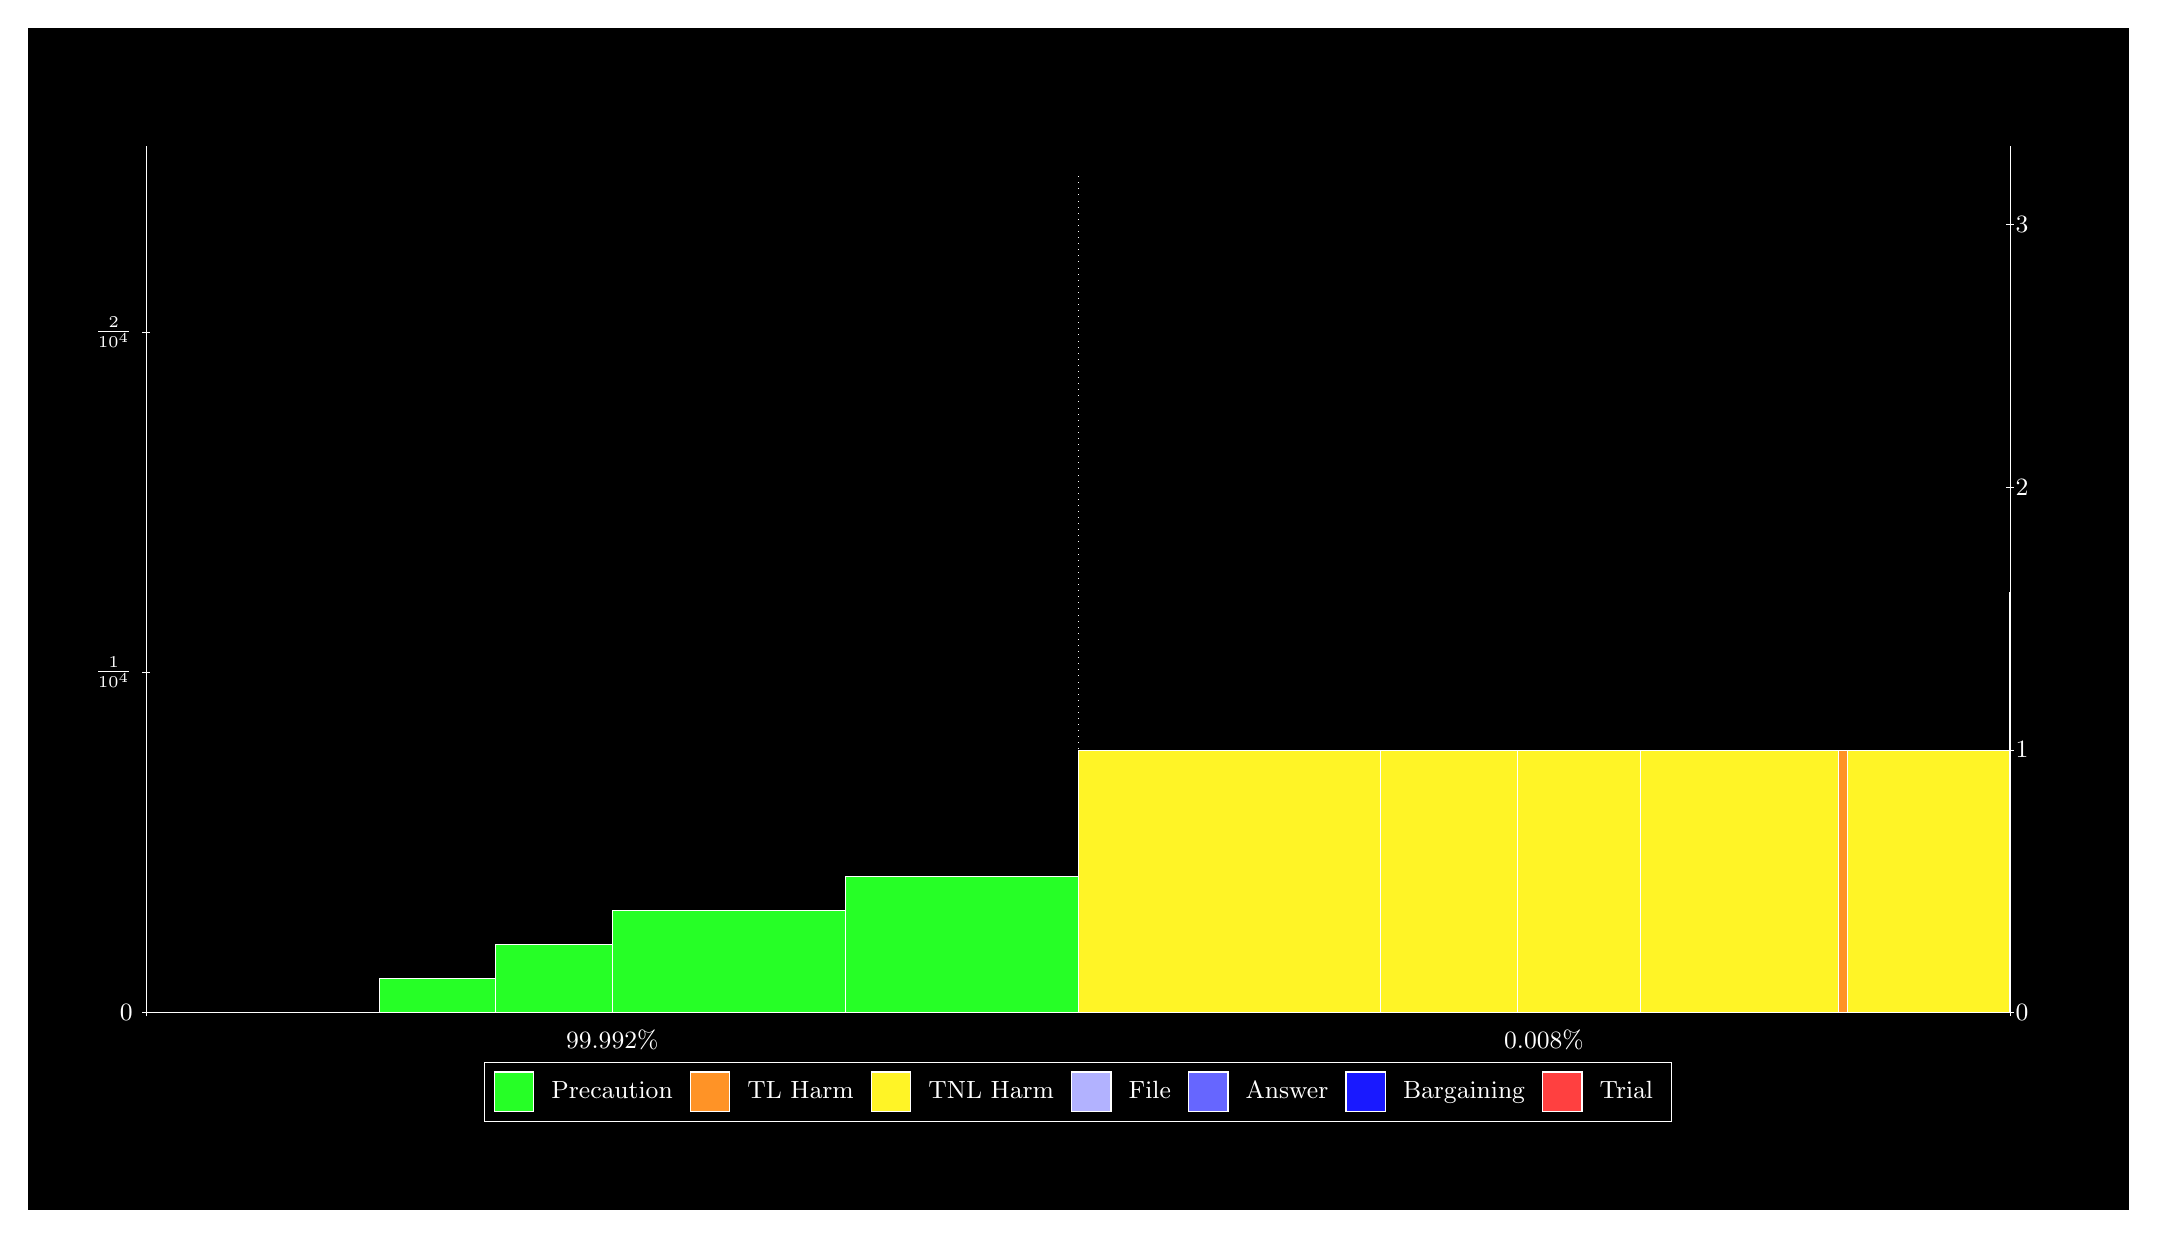
\begin{tikzpicture}
\draw[fill=black] (0,0) rectangle (26.667,15);
\draw[fill=green!85,draw=white,very thin] (4.4582,2.5) rectangle (5.9374,2.9321);
\draw[fill=green!85,draw=white,very thin] (5.9374,2.5) rectangle (7.4166,3.3641);
\draw[fill=green!85,draw=white,very thin] (7.4166,2.5) rectangle (10.375,3.7962);
\draw[fill=green!85,draw=white,very thin] (10.375,2.5) rectangle (13.333,4.2282);
\draw[fill=yellow!85,draw=white,very thin] (13.333,2.5) rectangle (17.165,5.8361);
\draw[fill=green!85,draw=white,very thin] (17.165,2.5) rectangle (18.914,2.5);
\draw[fill=yellow!85,draw=white,very thin] (17.165,2.5) rectangle (18.914,5.8361);
\draw[fill=green!85,draw=white,very thin] (18.914,2.5) rectangle (20.472,2.5001);
\draw[fill=yellow!85,draw=white,very thin] (18.914,2.5001) rectangle (20.472,5.8362);
\draw[fill=green!85,draw=white,very thin] (20.472,2.5) rectangle (22.983,2.5001);
\draw[fill=yellow!85,draw=white,very thin] (20.472,2.5001) rectangle (22.983,5.8362);
\draw[fill=green!85,draw=white,very thin] (22.983,2.5) rectangle (23.1,2.5001);
\draw[fill=orange!85,draw=white,very thin] (22.983,2.5001) rectangle (23.1,5.8362);
\draw[fill=green!85,draw=white,very thin] (23.1,2.5) rectangle (25.153,2.5001);
\draw[fill=yellow!85,draw=white,very thin] (23.1,2.5001) rectangle (25.153,5.8362);
\draw[fill=green!85,draw=white,very thin] (25.153,2.5) rectangle (25.167,2.5001);
\draw[fill=orange!85,draw=white,very thin] (25.153,2.5001) rectangle (25.167,5.8362);
\draw[fill=blue!30,draw=white,very thin] (25.153,5.8362) rectangle (25.167,6.1698);
\draw[fill=blue!60,draw=white,very thin] (25.153,6.1698) rectangle (25.167,6.5034);
\draw[fill=blue!90,draw=white,very thin] (25.153,6.5034) rectangle (25.167,7.1706);
\draw[fill=red!75,draw=white,very thin] (25.153,7.1706) rectangle (25.167,7.8378);
\draw[white,very thin] (1.5,2.5) -- (1.5,13.5);
\draw[white,very thin] (1.45,2.5) -- (1.55,2.5);
\node[font=\small,text=white, anchor=east] at (1.45, 2.5) {0};
\draw[white,very thin] (1.45,6.8206) -- (1.55,6.8206);
\node[font=\small,text=white, anchor=east] at (1.45, 6.8206) {$\frac{1}{10^{4}}$};
\draw[white,very thin] (1.45,11.141) -- (1.55,11.141);
\node[font=\small,text=white, anchor=east] at (1.45, 11.141) {$\frac{2}{10^{4}}$};

\draw[white,dotted,very thin] (13.333,2.83) -- (13.333,13.17);
\draw[white,very thin] (25.167,2.5) -- (25.167,13.5);
\draw[white,very thin] (25.117,2.5) -- (25.217,2.5);
\node[font=\small,text=white, anchor=west] at (25.117, 2.5) {0};
\draw[white,very thin] (25.117,5.8361) -- (25.217,5.8361);
\node[font=\small,text=white, anchor=west] at (25.117, 5.8361) {1};
\draw[white,very thin] (25.117,9.1722) -- (25.217,9.1722);
\node[font=\small,text=white, anchor=west] at (25.117, 9.1722) {2};
\draw[white,very thin] (25.117,12.508) -- (25.217,12.508);
\node[font=\small,text=white, anchor=west] at (25.117, 12.508) {3};

\draw[white,very thin] (1.5,2.5) -- (25.167,2.5);
\draw[white,very thin] (1.5,2.45) -- (1.5,2.55);
\node[font=\small,text=white, anchor=north] at (1.5, 2.45) {};
\draw[white,very thin] (25.167,2.45) -- (25.167,2.55);
\node[font=\small,text=white, anchor=north] at (25.167, 2.45) {};

\node[font=\small,text=white,anchor=south] at (7.4167, 1.9) {99.992\%};
\node[font=\small,text=white,anchor=south] at (19.25, 1.9) {0.008\%};
\draw (13.3333,2.5) node (B) {};
\begin{scope}[align=center]
\matrix[scale=0.5,draw=white,below=0.5cm of B,nodes={draw},column sep=0.1cm]{
\node[rectangle,draw,minimum width=0.5cm,minimum height=0.5cm,fill=green!85]{}; & \node[draw=none,font=\small,text=white]{Precaution}; &
\node[rectangle,draw,minimum width=0.5cm,minimum height=0.5cm,fill=orange!85]{}; & \node[draw=none,font=\small,text=white]{TL Harm}; &
\node[rectangle,draw,minimum width=0.5cm,minimum height=0.5cm,fill=yellow!85]{}; & \node[draw=none,font=\small,text=white]{TNL Harm}; &
\node[rectangle,draw,minimum width=0.5cm,minimum height=0.5cm,fill=blue!30]{}; & \node[draw=none,font=\small,text=white]{File}; &
\node[rectangle,draw,minimum width=0.5cm,minimum height=0.5cm,fill=blue!60]{}; & \node[draw=none,font=\small,text=white]{Answer}; &
\node[rectangle,draw,minimum width=0.5cm,minimum height=0.5cm,fill=blue!90]{}; & \node[draw=none,font=\small,text=white]{Bargaining}; &
\node[rectangle,draw,minimum width=0.5cm,minimum height=0.5cm,fill=red!75]{}; & \node[draw=none,font=\small,text=white]{Trial}; \\\\
};\end{scope}

\end{tikzpicture}
\end{document}